% Bismillahi-r-Rahmani-r-Rahim
\documentclass{article}
\author{Daoud Clarke}
\date{\today}
\title{Investigations into New Lattice Orderings}

\usepackage{color}
\usepackage{graphicx}
\usepackage{amssymb}
\usepackage[round]{natbib}

\newtheorem{definition}{Definition}

\newcommand{\R}{\mathbb{R}}

\begin{document}

\maketitle

Context-theoretic semantics \citep{Clarke:07} defines a lattice
ordering on the vector space formed from contexts of words. The
lattice meet and join are defined by taking component-wise minimums
and maximums with respect to the basis defined by contexts: there is a
basis vector (dimension) for each context a word can occur in.

However, this ordering is only one that is possible on the vector
space. Here we consider two others and evaluate their plausibility for
defining entailment between vector representations of meaning.

\section{Motivation}

In \citep{Clarke:12}, a context theory is defined as follows:
\begin{definition}[Context Theory]
A context theory is a tuple $\langle A, \mathcal{A}, \xi, V, \psi
\rangle$, where $A$ is a set (the alphabet), $\mathcal{A}$ is a unital
algebra over the real numbers, $\xi$ is a function from $A$ to
$\mathcal{A}$, $V$ is an abstract Lebesgue space and $\psi$ is an
injective linear map from $\mathcal{A}$ to $V$.
\end{definition}

The definition is quite complex because the space $V$ in which the
ordering is defined is a bigger space than the space $\mathcal{A}$
used to define composition. If we were able to define an ordering on
$\mathcal{A}$ instead, then this would significantly simplify the
definition, to $\langle A, \mathcal{A}, \xi\rangle$.

The second motivation for investigating new partial orderings is that
we can potentially learn them from data, instead of using a fixed
ordering defined by a basis. A partial ordering divides the space in a
similar way to the planes learnt by support vector machines, so it is
feasible that techniques from this area could be generalised to learn
cones.

\section{Background}

\begin{figure}
\begin{center}
%% Creator: Inkscape inkscape 0.48.0, www.inkscape.org
%% PDF/EPS/PS + LaTeX output extension by Johan Engelen, 2010
%% Accompanies image file 'basis.pdf' (pdf, eps, ps)
%%
%% To include the image in your LaTeX document, write
%%   \input{<filename>.pdf_tex}
%%  instead of
%%   \includegraphics{<filename>.pdf}
%% To scale the image, write
%%   \def\svgwidth{<desired width>}
%%   \input{<filename>.pdf_tex}
%%  instead of
%%   \includegraphics[width=<desired width>]{<filename>.pdf}
%%
%% Images with a different path to the parent latex file can
%% be accessed with the `import' package (which may need to be
%% installed) using
%%   \usepackage{import}
%% in the preamble, and then including the image with
%%   \import{<path to file>}{<filename>.pdf_tex}
%% Alternatively, one can specify
%%   \graphicspath{{<path to file>/}}
%% 
%% For more information, please see info/svg-inkscape on CTAN:
%%   http://tug.ctan.org/tex-archive/info/svg-inkscape

\begingroup
  \makeatletter
  \providecommand\color[2][]{%
    \errmessage{(Inkscape) Color is used for the text in Inkscape, but the package 'color.sty' is not loaded}
    \renewcommand\color[2][]{}%
  }
  \providecommand\transparent[1]{%
    \errmessage{(Inkscape) Transparency is used (non-zero) for the text in Inkscape, but the package 'transparent.sty' is not loaded}
    \renewcommand\transparent[1]{}%
  }
  \providecommand\rotatebox[2]{#2}
  \ifx\svgwidth\undefined
    \setlength{\unitlength}{188.26408691pt}
  \else
    \setlength{\unitlength}{\svgwidth}
  \fi
  \global\let\svgwidth\undefined
  \makeatother
  \begin{picture}(1,0.56574361)%
    \put(0,0){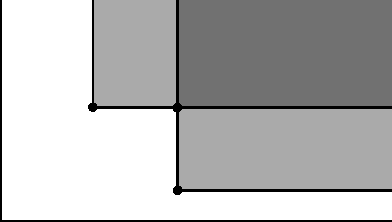
\includegraphics[width=\unitlength]{basis.pdf}}%
    \put(0.51254452,0.04251166){\color[rgb]{0,0,0}\makebox(0,0)[lb]{\smash{$u$}}}%
    \put(0.20261773,0.29920129){\color[rgb]{0,0,0}\makebox(0,0)[lb]{\smash{$v$}}}%
    \put(0.47721337,0.24375471){\color[rgb]{0,0,0}\makebox(0,0)[lb]{\smash{$u\lor v$}}}%
  \end{picture}%
\endgroup

\caption{The basis associated with a vector space can defines an
  ordering. This shows the join of two elements in the plane with the
  ordering defined by the basis formed from the $x$ and $y$ axes. The
  shaded areas are $u + C$ and $v + C$ where $C$ is the positive
  cone defined by this ordering. }
\end{center}
\end{figure}

A \textbf{partially ordered vector space} is a vector space $V$
together with a partial ordering $\le$ that satisfies:
\begin{itemize}
\item If $u \le v$ then $u + w \le v + w$
\item If $u \le v$ then $\alpha u \le \alpha v$
\end{itemize}
for all $u,v,w \in V$ and $\alpha \ge 0$. If the partial ordering is a
lattice, then the vector space is called a vector lattice or
\textbf{Riesz space}.

\begin{figure}
\begin{center}
%% Creator: Inkscape inkscape 0.48.0, www.inkscape.org
%% PDF/EPS/PS + LaTeX output extension by Johan Engelen, 2010
%% Accompanies image file 'cone.pdf' (pdf, eps, ps)
%%
%% To include the image in your LaTeX document, write
%%   \input{<filename>.pdf_tex}
%%  instead of
%%   \includegraphics{<filename>.pdf}
%% To scale the image, write
%%   \def\svgwidth{<desired width>}
%%   \input{<filename>.pdf_tex}
%%  instead of
%%   \includegraphics[width=<desired width>]{<filename>.pdf}
%%
%% Images with a different path to the parent latex file can
%% be accessed with the `import' package (which may need to be
%% installed) using
%%   \usepackage{import}
%% in the preamble, and then including the image with
%%   \import{<path to file>}{<filename>.pdf_tex}
%% Alternatively, one can specify
%%   \graphicspath{{<path to file>/}}
%% 
%% For more information, please see info/svg-inkscape on CTAN:
%%   http://tug.ctan.org/tex-archive/info/svg-inkscape

\begingroup
  \makeatletter
  \providecommand\color[2][]{%
    \errmessage{(Inkscape) Color is used for the text in Inkscape, but the package 'color.sty' is not loaded}
    \renewcommand\color[2][]{}%
  }
  \providecommand\transparent[1]{%
    \errmessage{(Inkscape) Transparency is used (non-zero) for the text in Inkscape, but the package 'transparent.sty' is not loaded}
    \renewcommand\transparent[1]{}%
  }
  \providecommand\rotatebox[2]{#2}
  \ifx\svgwidth\undefined
    \setlength{\unitlength}{259.341008pt}
  \else
    \setlength{\unitlength}{\svgwidth}
  \fi
  \global\let\svgwidth\undefined
  \makeatother
  \begin{picture}(1,0.63246843)%
    \put(0,0){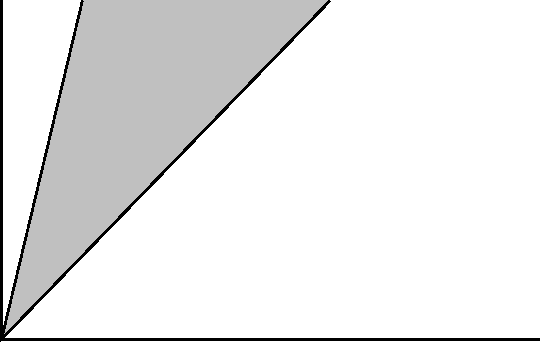
\includegraphics[width=\unitlength]{cone.pdf}}%
  \end{picture}%
\endgroup

\end{center}
\caption{A cone $C$ defining a lattice ordering on the two dimensional
  vector space in the plane.}
\end{figure}

\begin{figure}
\begin{center}
%% Creator: Inkscape inkscape 0.48.0, www.inkscape.org
%% PDF/EPS/PS + LaTeX output extension by Johan Engelen, 2010
%% Accompanies image file 'cones.pdf' (pdf, eps, ps)
%%
%% To include the image in your LaTeX document, write
%%   \input{<filename>.pdf_tex}
%%  instead of
%%   \includegraphics{<filename>.pdf}
%% To scale the image, write
%%   \def\svgwidth{<desired width>}
%%   \input{<filename>.pdf_tex}
%%  instead of
%%   \includegraphics[width=<desired width>]{<filename>.pdf}
%%
%% Images with a different path to the parent latex file can
%% be accessed with the `import' package (which may need to be
%% installed) using
%%   \usepackage{import}
%% in the preamble, and then including the image with
%%   \import{<path to file>}{<filename>.pdf_tex}
%% Alternatively, one can specify
%%   \graphicspath{{<path to file>/}}
%% 
%% For more information, please see info/svg-inkscape on CTAN:
%%   http://tug.ctan.org/tex-archive/info/svg-inkscape

\begingroup
  \makeatletter
  \providecommand\color[2][]{%
    \errmessage{(Inkscape) Color is used for the text in Inkscape, but the package 'color.sty' is not loaded}
    \renewcommand\color[2][]{}%
  }
  \providecommand\transparent[1]{%
    \errmessage{(Inkscape) Transparency is used (non-zero) for the text in Inkscape, but the package 'transparent.sty' is not loaded}
    \renewcommand\transparent[1]{}%
  }
  \providecommand\rotatebox[2]{#2}
  \ifx\svgwidth\undefined
    \setlength{\unitlength}{259pt}
  \else
    \setlength{\unitlength}{\svgwidth}
  \fi
  \global\let\svgwidth\undefined
  \makeatother
  \begin{picture}(1,0.71832129)%
    \put(0,0){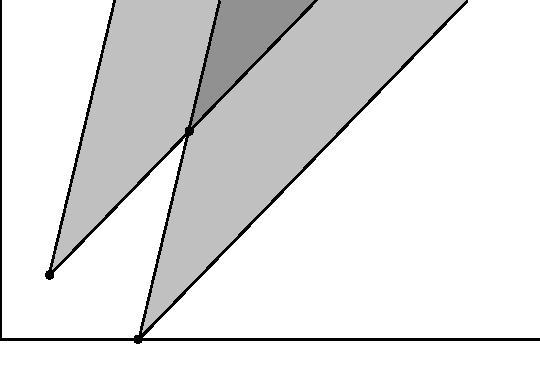
\includegraphics[width=\unitlength]{cones.pdf}}%
    \put(0.0289539,0.14386651){\color[rgb]{0,0,0}\makebox(0,0)[lb]{\smash{$u$}}}%
    \put(0.20731187,0.01815878){\color[rgb]{0,0,0}\makebox(0,0)[lb]{\smash{$v$}}}%
    \put(0.32271158,0.41831799){\color[rgb]{0,0,0}\makebox(0,0)[lb]{\smash{$u\lor v$}}}%
  \end{picture}%
\endgroup

\end{center}
\caption{The join of two elements $u$ and $v$ and the spaces $u + C$
  and $v + C$ where $C$ is the cone defining the ordering of the
  space.}
\end{figure}

A \textbf{cone} is a subset $C$ of a vector space satisfying
\begin{itemize}
\item $C + C \subseteq C$
\item $\alpha C \subseteq C$ for all $\alpha \ge 0$
\item $C \cap (-C) = \{0\}$
\end{itemize}
If $V$ is a partially ordered vector space, then the set $V^+ = \{v
\in V : v \ge 0\}$ is a cone, called the \textbf{positive
  cone}. Conversely, given any cone $C$ for a vector space $V$, we can
define a partial ordering on $V$ by $u \le v$ iff $v - u \in C$.

Given a countable set $U = \{u_1, u_2, \ldots\}$ of vectors, the cone
generated by $U$ is the set $C_U = \{v : v = \sum_i \alpha_i u_i\}$ for
some $\alpha_i \ge 0$.

\section{Context Vector Cones}

We can define a positive cone on $\mathcal{A}$ to be the cone
generated by all context vectors, $\hat{A} = \{\hat{x} : x \in A^*\}$. There are
two questions we can ask:
\begin{itemize}
\item Is the ordering interesting, or is likely to turn out to be
  trivial (for example, all strings have meet $0$)?
\item Does the ordering define a lattice? We need the meet operation
in order to define a degree of entailment between strings.
\end{itemize}

In fact it seems that we can't have our cake and eat it, as if the
first question is true, it seems likely the second is false, and vice
versa. If the set $\hat{A}$ is linearly independent, then it seems
that the first is true, and the second false, while the converse holds
in general otherwise. (At the moment, I only have an intuition for
this --- I've yet to prove it).


\section{Plane Orderings}

\begin{figure}
\begin{center}
%% Creator: Inkscape inkscape 0.48.0, www.inkscape.org
%% PDF/EPS/PS + LaTeX output extension by Johan Engelen, 2010
%% Accompanies image file 'plane.pdf' (pdf, eps, ps)
%%
%% To include the image in your LaTeX document, write
%%   \input{<filename>.pdf_tex}
%%  instead of
%%   \includegraphics{<filename>.pdf}
%% To scale the image, write
%%   \def\svgwidth{<desired width>}
%%   \input{<filename>.pdf_tex}
%%  instead of
%%   \includegraphics[width=<desired width>]{<filename>.pdf}
%%
%% Images with a different path to the parent latex file can
%% be accessed with the `import' package (which may need to be
%% installed) using
%%   \usepackage{import}
%% in the preamble, and then including the image with
%%   \import{<path to file>}{<filename>.pdf_tex}
%% Alternatively, one can specify
%%   \graphicspath{{<path to file>/}}
%% 
%% For more information, please see info/svg-inkscape on CTAN:
%%   http://tug.ctan.org/tex-archive/info/svg-inkscape

\begingroup
  \makeatletter
  \providecommand\color[2][]{%
    \errmessage{(Inkscape) Color is used for the text in Inkscape, but the package 'color.sty' is not loaded}
    \renewcommand\color[2][]{}%
  }
  \providecommand\transparent[1]{%
    \errmessage{(Inkscape) Transparency is used (non-zero) for the text in Inkscape, but the package 'transparent.sty' is not loaded}
    \renewcommand\transparent[1]{}%
  }
  \providecommand\rotatebox[2]{#2}
  \ifx\svgwidth\undefined
    \setlength{\unitlength}{208.96237793pt}
  \else
    \setlength{\unitlength}{\svgwidth}
  \fi
  \global\let\svgwidth\undefined
  \makeatother
  \begin{picture}(1,0.74643873)%
    \put(0,0){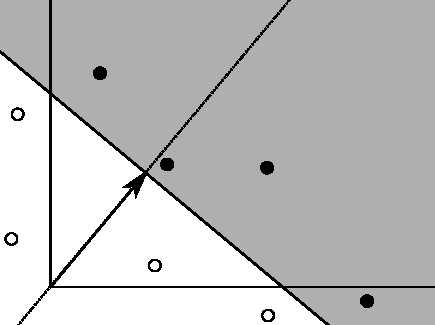
\includegraphics[width=\unitlength]{plane.pdf}}%
    \put(0.2592593,0.20904595){\color[rgb]{0,0,0}\makebox(0,0)[lb]{\smash{$p$}}}%
    \put(0.49585026,0.47787869){\color[rgb]{0,0,0}\makebox(0,0)[lb]{\smash{$\hat{p}$}}}%
  \end{picture}%
\endgroup

\end{center}
\caption{A plane found using a support vector machine can be
  considered as dividing the vector space, and thus defines a partial
  ordering.}
\end{figure}

There is an interesting similarity between how a cone divides the
vector space and the division of a space introduced by a plane, as
used for example in support vector machines. In fact the plane also
defines an ordering, if we define one side to be ``positive''. Then,
as before, $x \le y$ if $y - x$ is on the positive side of the plane.

The ordering is determined entirely by the dimension perpendicular to
the plane. Let $p$ be the vector from the origin to the plane, and
perpendicular to it, and $\bar{p}$ be the one dimensional subspace
generated by $p$. Then $x \le y$ iff $\|\hat{p}(y) - \hat{p}(x)\| \ge
\|p\|$, where by $\hat{p}(x)$ we mean the projection of $x$ onto the
dimension $\hat{p}$, that is, if the projection of $y - x$ onto the
subspace generated by $p$ is greater than or equal to $p$.

In general, this ordering is not a vector space ordering as defined
above unless it passes through the origin. The zero vector is either
positive or negative depending on which side of the plane it
falls. It also does not define a lattice ordering. For example, when
the plane does pass through the origin, the plane defines a total
ordering between vectors purely depending on their position when
projected onto $\hat{p}$. Any vectors on the plane perpendicular to a
point on $\hat{p}$ are equivalent under this partial ordering (thus it
is not strictly a partial ordering).

\section{Relating Strings of Different Lengths with Orderings}

We can use vector space orderings to relate strings of different
lengths. This is similar to the quotient algebra construction of
\cite{Clarke:10}, but allows us to specify the asymmetric relation of
entailment, instead of equating vectors. In fact the two techniques
complement one another: if we need to impose equality between vectors
we can use the quotient algebra construction, and if we need to relate
two vectors by entailment then we can change the ordering.

For example, if we wish to impose the conjunctive nature of ``and'' on
the vector space, we can do this by requiring that $uav \le u$ and
$uav \le v$ for all $u$ and $v$ where $a$ is the vector for
``and''. We can do the same for ``or'' with $u \le uov$ and $v\le uov$
where $o$ is the vector for ``or''.

Similarly, we can make all adjectives restrict the properties of the
nouns they operate on by making $au \le u$ for all adjective vectors
$a$ and all noun space vectors $u$.

In a sense, this is like imposing a logic on top of the vector space
structure, where the rules of the logic are encapsulated in the
positive cone.

\subsection{Application to Sentence Space}

This also gives us a surprising answer for what the sentence space
should look like: it doesn't really matter, as long as the ordering
between sentences can be specified correctly. For example, we can just
use the tensor product between sentences but ensure that $s_1\otimes s_2 \le
s_1$ and $s_1\otimes s_2\le s_2$.

Let $V$ be a fixed dimensional space used to represent the meaning of
a single sentence, then we use
$$T(V) = \mathbb{R}\oplus V \oplus (V\otimes V) \oplus (V\otimes V\otimes V) \oplus \cdots$$
to represent multiple sentences. Given a partial ordering $\le$ on
$V$, there is a natural extension to an ordering on $T(V)$, for
example $u_1\otimes v_1 \le u_2\otimes v_2$ iff $u_1 \le u_2$ and
$v_1 \le v_2$, and similarly for higher tensor powers.

We also assume that $V$ has a preferred basis that defines a natural
lattice ordering, by $u_1 \le u_2$ if every component of $u_1$ is less
than or equal to the corresponding component of $u_2$.

Let $C$ be the positive cone on $T(V)$ as defined above, i.e.~the set
of all vectors $u\in T(V)$ such that $u \ge 0$. Under the standard
ordering, strings of different lengths are not related, so we add
additional vectors to $C$ to relate them. Let
$$C' = C \cup \{ u - u\otimes v : u,v \in C \} \cup \{ v - u\otimes v : u,v \in C \}$$
This defines a cone which behaves as the normal ordering for strings
of the same length, but allows strings of different lengths to be
related.

\subsection{Problems with this Ordering}

There is freedom in choosing elements which allows the whole
half-plane to be generated. For example in $u - u\otimes v$, $v$ can
be a very large positive vector, or $u$ very small, and in the limit,
this is the same as adding $-u\otimes v$ to the positive cone which
leads to an uninteresting ordering.

% To get around this we can try and limit the size of vectors we add:
% $$D = \{ u - u\otimes v : u,v \in U(C) \} \cup \{ v - u\otimes v : u,v \in U(C) \}$$
% where $U(C)$ denotes the set of all vectors $u\in C$ with $\|u\| = 1$,
% then generate the new positive cone $C'$ from $D\cup C$.

\subsection{Basis Orderings}

Write $V^{\otimes n}$ for the subspace of $T(V)$ generated by tensor
powers of $V$ to the $n$th degree, and $T^n(V)$ for the subspace
generated by all tensor powers up to and including $n$.

Let $B = \{e_1, e_2, \ldots\}$ be an orthonormal basis for
$T(V)$. Assume for each basis vector $e_i$ in $T(V)$, if $e_i\in
V^{\otimes n}$ we have a vector $u_i \in T^{n-1}(V) \cap C$.

We then define a new cone $D$ to be that generated by
$$\{e_i - u_i\ : i \ge 1\} \cup B$$

\subsection{Example from Quotient Algebra}

Plain tensor algebra:

\begin{tabular}{llllllllll}
term & red book &  city &  apple & big city & red apple & big book &  book & big apple & red city\\ 
red book & 1 & 0 & 0 & 0 & 0.33 & 1 & 0 & 0.33 & 0\\ 
 city & 0 & 1 & 0.33 & 0 & 0 & 0 & 0 & 0 & 0\\ 
 apple & 0 & 0.33 & 1 & 0 & 0 & 0 & 0.33 & 0 & 0\\ 
big city & 0 & 0 & 0 & 1 & 0.22 & 0 & 0 & 0.33 & 0.67\\ 
red apple & 0.33 & 0 & 0 & 0.33 & 1 & 0.33 & 0 & 1 & 0.33\\ 
big book & 0.67 & 0 & 0 & 0 & 0.22 & 1 & 0 & 0.33 & 0\\ 
 book & 0 & 0 & 0.33 & 0 & 0 & 0 & 1 & 0 & 0\\ 
big apple & 0.22 & 0 & 0 & 0.33 & 0.67 & 0.33 & 0 & 1 & 0.22\\ 
red city & 0 & 0 & 0 & 1 & 0.33 & 0 & 0 & 0.33 & 1\\ 
\end{tabular}

Cone:

\begin{tabular}{llllllllll}
term & red book &  city &  apple & big city & red apple & big book &  book & big apple & red city\\ 
red book & 1 & 0 & 0.11 & 0 & 0.33 & 1 & 0.33 & 0.33 & 0\\ 
 city & 0 & 1 & 0.33 & 1 & 0.33 & 0 & 0 & 0.33 & 1\\ 
 apple & 0.33 & 0.33 & 1 & 0.33 & 1 & 0.33 & 0.33 & 1 & 0.33\\ 
big city & 0 & 0.25 & 0.083 & 1 & 0.25 & 0 & 0 & 0.33 & 0.75\\ 
red apple & 0.33 & 0.11 & 0.33 & 0.33 & 1 & 0.33 & 0.11 & 1 & 0.33\\ 
big book & 0.75 & 0 & 0.083 & 0 & 0.25 & 1 & 0.25 & 0.33 & 0\\ 
 book & 1 & 0 & 0.33 & 0 & 0.33 & 1 & 1 & 0.33 & 0\\ 
big apple & 0.25 & 0.083 & 0.25 & 0.33 & 0.75 & 0.33 & 0.083 & 1 & 0.25\\ 
red city & 0 & 0.33 & 0.11 & 1 & 0.33 & 0 & 0 & 0.33 & 1\\ 
\end{tabular}

\bibliographystyle{plainnat}

\bibliography{contexts}

\end{document}
